\documentclass[10pt]{extarticle}
\usepackage[a4paper,margin=1.5cm,columnsep=0.7cm]{geometry}
\usepackage{amsmath,amssymb}
\usepackage{graphicx}
\usepackage{enumitem}
\usepackage{booktabs}
\usepackage{array}
\usepackage{tabularx}
\usepackage[T1]{fontenc}
\usepackage{multicol}

\setlength{\parindent}{0pt}
\setlength{\parskip}{4pt}
\renewcommand{\arraystretch}{1.15}

\newenvironment{qoptions}{\begin{itemize}[leftmargin=1.8em,itemsep=2pt,topsep=2pt,label={}]}{\end{itemize}}
\newcommand{\opt}[2]{\item[({#1})] {#2}}

\newcommand{\sectionhdr}[1]{\par\vspace{4pt}\noindent\textbf{\large #1}\par\vspace{2pt}}
\newcommand{\subsectionhdr}[1]{\par\vspace{3pt}\noindent\textbf{#1}\par\vspace{2pt}}

\pagestyle{empty}

\begin{document}
\begin{center}
{\LARGE\bfseries JEE (Main+Advanced) Score-II --- Test 32 (29 Mar 2024)}
\end{center}
\vspace{6pt}

\begin{multicols}{2}

\sectionhdr{PART-1: PHYSICS}
\subsectionhdr{Section-I (i): Single Correct}

\textbf{1.} A rod of length $\ell$ = 1 m and cross sectional area $1.0\times10^{-3}$ m$^2$ is floating in the water as shown in the figure. Centre of mass of the rod is 20 cm from its lower end and 80\% of the rod is dipped in water in equilibrium. The rod is tilted slightly from its vertical position about center of mass and released. The subsequent motion is observed to be SHM. Moment of inertia of the rod about the center of mass is 0.4 Kg-m$^2$. The time period of the oscillation will be-

\begin{center}
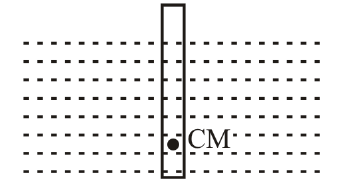
\includegraphics[width=0.55\linewidth]{Score-II - Test 32 (29 Mar 2024)-img/p1phy_q1_rod.png}
\end{center}

\begin{qoptions}
\opt{A}{$\pi$ sec}
\opt{B}{$\dfrac\pi4$ sec}
\opt{C}{$\dfrac\pi8$ sec}
\opt{D}{$\dfrac\pi2$ sec}
\end{qoptions}

\textbf{2.} A system consists of two identical blocks, each of mass m = 0.1 kg linked together by the compressed weightless spring of spring constant K = 50 N/m of initial compression 8 cm. The blocks are also connected by a thread which is burned through at a certain moment, what will be the velocity of upper block at the moment when lower block has just left the surface?

\begin{center}
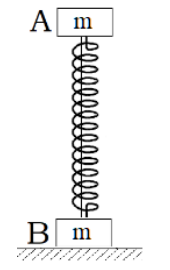
\includegraphics[width=0.3\linewidth]{Score-II - Test 32 (29 Mar 2024)-img/p1phy_q2_spring.png}
\end{center}

\begin{qoptions}
\opt{A}{1 m/s}
\opt{B}{2 m/s}
\opt{C}{3 m/s}
\opt{D}{4 m/s}
\end{qoptions}

\textbf{3.} Three identical biconvex lenses of focal length f are aligned with two neighbouring lenses separated by a distance f as shown in the figure. A small object is located at a distance f/2 in front of the leftmost lens. Choose the correct option.

\begin{center}
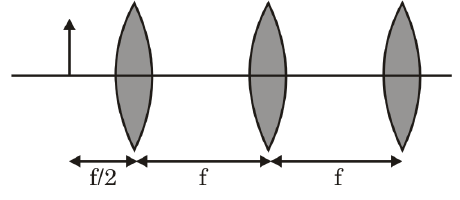
\includegraphics[width=0.9\linewidth]{Score-II - Test 32 (29 Mar 2024)-img/p1phy_q3_lenses.png}
\end{center}

\begin{qoptions}
\opt{A}{The final image formed is real and inverted.}
\opt{B}{The final image formed is virtual and erect.}
\opt{C}{The final image formed is real \& erect.}
\opt{D}{The final image formed is virtual and inverted.}
\end{qoptions}

\textbf{4.} A triangular shaped pulse of length L is completely reflected at the fixed end of the string on which it travels. What will be the shape of the pulse after a length $\dfrac{3L}4$ of the pulse has been reflected?

\begin{center}
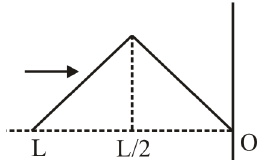
\includegraphics[width=0.55\linewidth]{Score-II - Test 32 (29 Mar 2024)-img/p1phy_q4_initial.png}
\end{center}

\begin{center}
\begin{minipage}{0.47\linewidth}
\centering
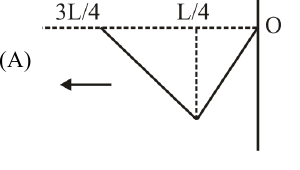
\includegraphics[width=0.9\linewidth]{Score-II - Test 32 (29 Mar 2024)-img/p1phy_q4_A.png}
\end{minipage}
\begin{minipage}{0.47\linewidth}
\centering
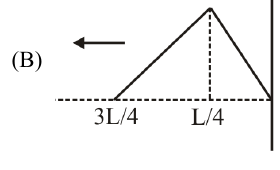
\includegraphics[width=0.9\linewidth]{Score-II - Test 32 (29 Mar 2024)-img/p1phy_q4_B.png}
\end{minipage}

\begin{minipage}{0.47\linewidth}
\centering
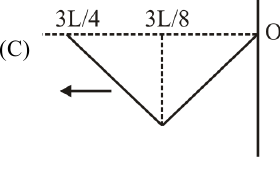
\includegraphics[width=0.9\linewidth]{Score-II - Test 32 (29 Mar 2024)-img/p1phy_q4_C.png}
\end{minipage}
\begin{minipage}{0.47\linewidth}
\centering
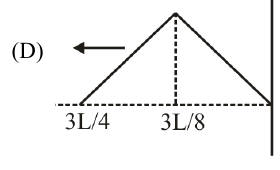
\includegraphics[width=0.9\linewidth]{Score-II - Test 32 (29 Mar 2024)-img/p1phy_q4_D.png}
\end{minipage}
\end{center}

\subsectionhdr{Section-I (ii): One or more correct}

\textbf{5.} A streamline curvilinear flow exihibits circular curvature on a horizontal plane as shown in figure. At radius of curvature r$_1$ the velocity of stream is v$_1$ and pressure p$_1$ and another radius of curvature r$_2$ the velocity of stream is v$_2$ and pressure p$_2$. Choose the correct options

\begin{center}
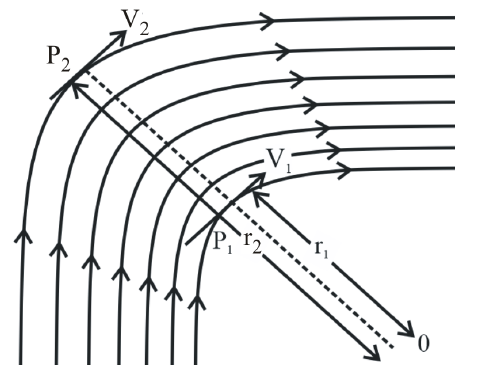
\includegraphics[width=0.85\linewidth]{Score-II - Test 32 (29 Mar 2024)-img/p1phy_q5_flow.png}
\end{center}

\begin{qoptions}
\opt{A}{p$_2$ > p$_1$}
\opt{B}{v$_2$ > v$_1$}
\opt{C}{$\dfrac{v_1^2}{r_1}=\dfrac{v_2^2}{r_2}$}
\opt{D}{v$_1$r$_1$ = v$_2$r$_2$}
\end{qoptions}

\textbf{6.} Consider a uniformly charged non conducting spherical shell of radius R. Net charge on the shell is Q (Q > 0). There is a small hole in the shell at `A' shown in the figure. The shell and a point charge $-q$ (q > 0) are released at a separation 2R from the center as shown in the figure. The shell and point charge have same mass m. After release, the point charge will move toward shell, passes through the hole and hit the shell at `B'. (consider $k=\dfrac1{4\pi\epsilon_0}$). Choose the correct option(s):

\begin{center}
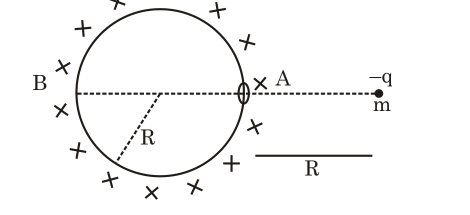
\includegraphics[width=0.85\linewidth]{Score-II - Test 32 (29 Mar 2024)-img/p1phy_q6_shell.png}
\end{center}

\begin{qoptions}
\opt{A}{The distance travelled by point charge till it hits the shell at B is $\dfrac{5R}2$.}
\opt{B}{Speed of the point charge when it hits the shell is $\sqrt{\dfrac{kQq}{2mR}}$.}
\opt{C}{Time taken by the point charge to travel from A to B is $\sqrt{\dfrac{8mR^3}{kQq}}$.}
\opt{D}{The distance travelled by the shell till the collision is R.}
\end{qoptions}

\textbf{7.} As shown in figure a parallel plate capacitor is composed of two circular plates with a radius of r. The gap d between the two plates is very small. The two plates are charged $+Q_0$ and $-Q_0$ respectively. At t = 0, use a thin straight wire with resistance R to connect the centers of the plates. Assume that the resistance R is very large, so that the electric field between the two plates remains uniform at any time, and the inductance can be ignored. $\left(\dfrac{\epsilon_0\pi r^2}d=C\right)$

\begin{center}
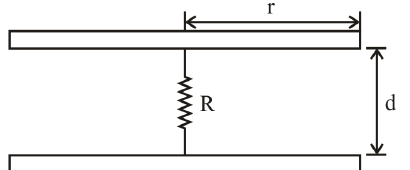
\includegraphics[width=0.75\linewidth]{Score-II - Test 32 (29 Mar 2024)-img/p1phy_q7_capacitor.png}
\end{center}

\begin{qoptions}
\opt{A}{Charge on capacitor as function of time is Q$_0$e$^{-t/RC}$.}
\opt{B}{The net current passing through a ring of radius $\rho\ (\rho<r)$ coaxial with the capacitor as a function of time is $\dfrac{Q_0}{RC}e^{-t/RC}$.}
\opt{C}{The net current passing through a ring of radius $\rho\ (\rho>r)$ coaxial with the capacitor as a function of time is $\dfrac{Q_0}{RC}e^{-t/RC}$.}
\opt{D}{The magnetic field at a distance $\rho\ (\rho<r)$ from the axis of the capacitor at any time t is $\dfrac{\mu_0}{2\pi\rho}\left(1-\dfrac{\rho^2}{r^2}\right)\dfrac{Q_0}{RC}e^{-t/RC}$.}
\end{qoptions}

\subsectionhdr{Section-II (i): Paragraph-based Numerical}

\textbf{Paragraph for Questions 1 and 2}

A solid cubical box of side a and mass m moves down an inclined plane with a constant velocity V$_0$. The inclination of the plane with horizontal is $\theta=15^\circ$. The bottom of the incline plane is joined with a horizontal plane at point (S) as shown in figure. The corner B of the box hit the corner (S) perfectly inelastically, causing the box to topple about the corner B. The velocity of the centre of the box immediately after collision is V. Answer the following questions

\begin{center}
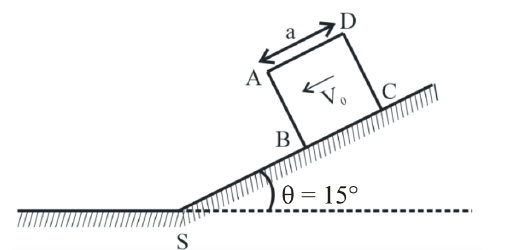
\includegraphics[width=0.7\linewidth]{Score-II - Test 32 (29 Mar 2024)-img/p1phy_n12_incline.png}
\end{center}

\textbf{1.} Find V (in m/s) if V$_0=4\sqrt2$ m/s.

\textbf{2.} Find the minimum value of V$_0^2$ in (SI unit) such that the cubical box topples about the bottom edge B at corner S. (Take: $a=\dfrac{3\sqrt2(2+\sqrt3)}{320}$ m)

\textbf{Paragraph for Questions 3 and 4}

An unknown Nucleus (x) can decay into other nucleus (y) by two decay schemes shown in figure.
(i) It can emit a $\beta$ particle ($\beta_1$) and come to ground state by either emitting one $\gamma$ ray($\gamma_1$) or emitting two $\gamma$ rays ($\gamma_3$ \& $\gamma_2$)
(ii) It can emit one $\beta$ particle ($\beta_2$) and come to ground state by emitting $\gamma_2$ ray. Atomic masses: x = 197.9682 amu, y = 197.9662 amu, 1 amu = 930 MeV/c$^2$. The energy levels of the nucleus are shown in figure.

\begin{center}
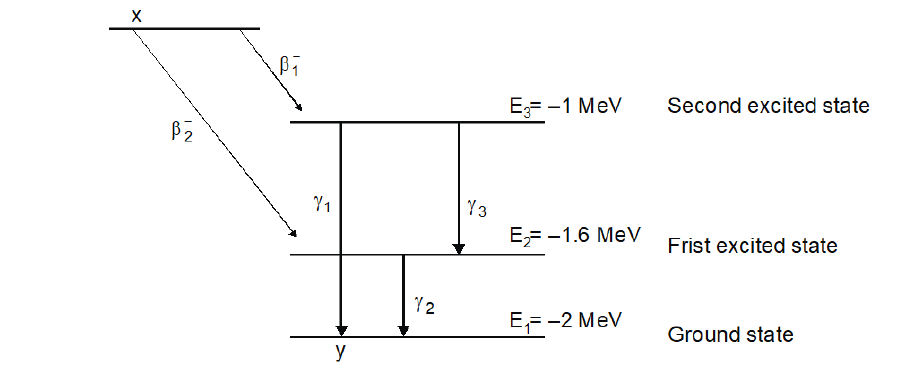
\includegraphics[width=0.95\linewidth]{Score-II - Test 32 (29 Mar 2024)-img/p1phy_n34_decay.png}
\end{center}

\textbf{3.} What is the maximum kinetic energy of emitted $\beta_2$ particle? (in MeV)

\textbf{4.} What is the maximum kinetic energy of emitted $\beta_1$ particle? (in MeV)

\subsectionhdr{Section-II (ii): Non-negative Integer}

\textbf{5.} In the L--C circuit, the capacitor C$_1$ is charged to a potential of 1 volt, and the capacitor C$_2$ and the inductor were initially uncharged. Now switch S$_1$ is closed at t = 0, and at $t=\dfrac{1.5\pi}{100}$ sec. switch S$_2$ is closed and S$_1$ is opened simultaneously. Further after $\dfrac{0.5\pi}{100}$ sec., S$_2$ is also opened. Find final potential difference across the capacitor C$_2$ in volt.

\begin{center}
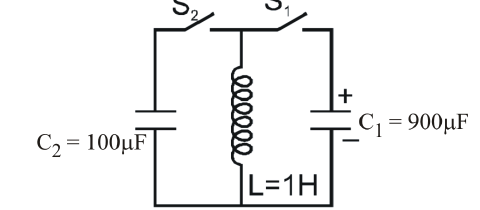
\includegraphics[width=0.75\linewidth]{Score-II - Test 32 (29 Mar 2024)-img/p1phy_n5_lc.png}
\end{center}

\textbf{6.} A thin hollow cylinder (opened at the both ends) of radius and length both equal to L. This object carries a uniform surface-charge density $\sigma$. The electrostatic potential at the point P on the axis of the cylinder (as shown in the figure) comes out to be $V_P=\dfrac{\sigma L}{k\varepsilon_0}\ell n(1+\sqrt h)$. Find the value of (k + h).

\begin{center}
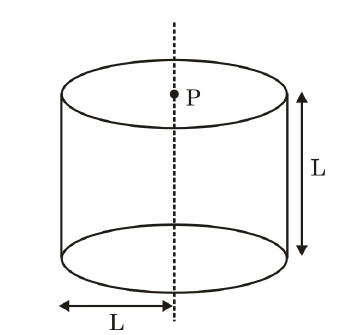
\includegraphics[width=0.55\linewidth]{Score-II - Test 32 (29 Mar 2024)-img/p1phy_n6_cylinder.png}
\end{center}

\textbf{7.} A cylindrical rod of length 64 cm and cross-section radius $r=\left(\dfrac2{\sqrt\pi}\right)$ cm is placed at a distance 50r from a infrared point source S of power 1.25 kW as shown in the figure. The lateral surface of the rod is perfectly insulated from the surroundings. The cross-section A absorbs 80\% of the incident energy, has temperature T$_A$ in steady state. The surface B is radiating energy into space and the wavelength emitted by it with maximum energy density is 100,000 \AA. Find the value T$_A$ (temperature of end A in Kelvin) if conductivity varies with temp as $K=\dfrac{T}{T_A}$. Assume that the rate of flow of heat through the rod is steady. Wein's constant = 0.003 mK).

\begin{center}
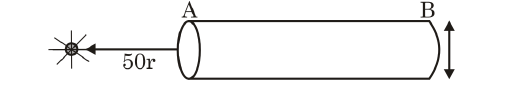
\includegraphics[width=0.85\linewidth]{Score-II - Test 32 (29 Mar 2024)-img/p1phy_n7_rod.png}
\end{center}

\textbf{8.} 12 capacitors are connected with a battery of potential difference V$_0$ as shown in the figure. Initially switch is open. The total heat generated in the system after the switch is closed is $\alpha\times10^{-8}$ J. The value of $\alpha$ is:- (Given $C=\dfrac1{340}\mu$F, V$_0$ = 17 volt)

\begin{center}
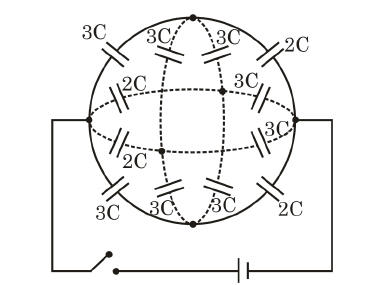
\includegraphics[width=0.65\linewidth]{Score-II - Test 32 (29 Mar 2024)-img/p1phy_n8_capacitors.png}
\end{center}

\textbf{9.} Find the magnitude of entropy change for n = 2.0 moles of an ideal gas whose adiabatic exponent $\gamma$ = 1.30 if, as a result of a certain process, the gas volume increased $\alpha$ = 2.0 times while the pressure dropped $\beta$ = 3.0 times. (ln2 = 0.7, ln3 = 1.1), Round off to nearest integer.

\textbf{10.} One mole of an ideal monoatomic gas is taken through a thermodynamic process shown in the P-V diagram, where AB is a semi circular arc. The heat supplied to the system in this process is $(\pi+\alpha)P_0V_0$. The value of $\alpha$ is

\begin{center}
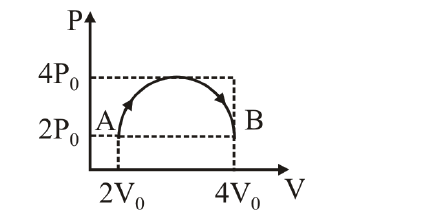
\includegraphics[width=0.6\linewidth]{Score-II - Test 32 (29 Mar 2024)-img/p1phy_n10_pv.png}
\end{center}

\sectionhdr{PART-2: CHEMISTRY}
\subsectionhdr{Section-I (i): Single Correct}

\textbf{1.} Treatment of D-glucose with aqueous NaOH results in a mixture of monosaccharides, which are

\end{multicols}
\begin{center}
\begin{minipage}{0.47\linewidth}\centering\textbf{(A)}\\[2pt]
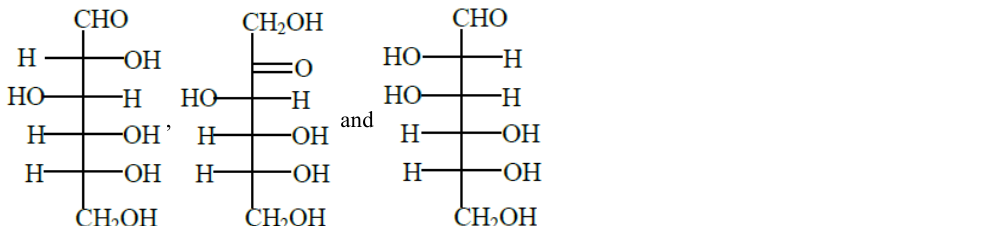
\includegraphics[width=0.95\linewidth]{Score-II - Test 32 (29 Mar 2024)-img/q1_A.png}
\end{minipage}\hfill
\begin{minipage}{0.47\linewidth}\centering\textbf{(B)}\\[2pt]
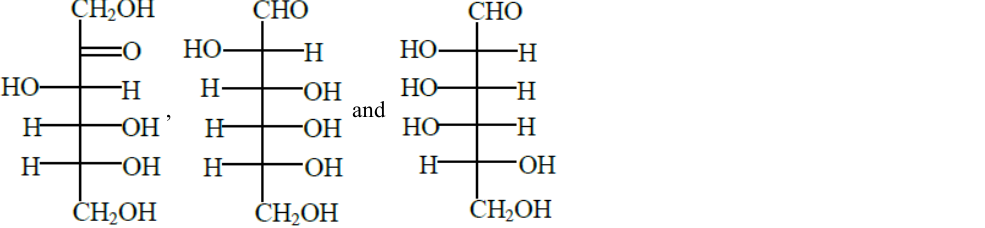
\includegraphics[width=0.95\linewidth]{Score-II - Test 32 (29 Mar 2024)-img/q1_B.png}
\end{minipage}

\vspace{6pt}
\begin{minipage}{0.47\linewidth}\centering\textbf{(C)}\\[2pt]
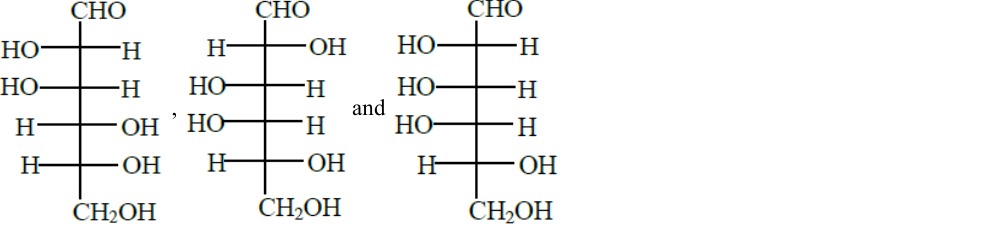
\includegraphics[width=0.95\linewidth]{Score-II - Test 32 (29 Mar 2024)-img/q1_C.png}
\end{minipage}\hfill
\begin{minipage}{0.47\linewidth}\centering\textbf{(D)}\\[2pt]
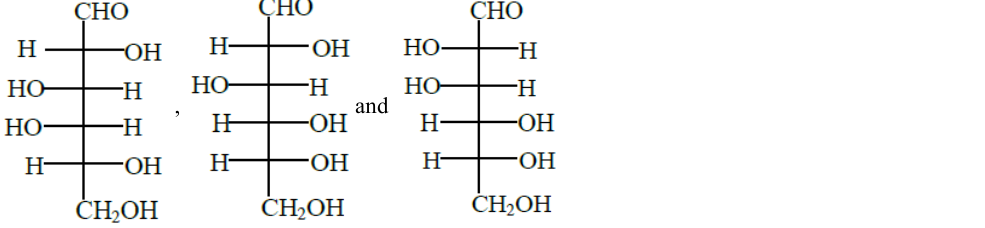
\includegraphics[width=0.95\linewidth]{Score-II - Test 32 (29 Mar 2024)-img/q1_D.png}
\end{minipage}
\end{center}
\begin{multicols}{2}

\textbf{2.} If Bauxite contains SiO$_2$, iron oxides, TiO$_2$ as impurities and leaching agent is conc. NaOH then which of the following option is correct for Bayer process?

\begin{qoptions}
\opt{A}{In digestion, Al$_2$O$_3$ is extracted out as hydrated alumina.}
\opt{B}{In this process H$_2$S(g) is used for the neutralisation of solution.}
\opt{C}{After seeding precipitation of Alumina decreases.}
\opt{D}{In this process one of the product will be NaHCO$_3$.}
\end{qoptions}

\textbf{3.} NaIO$_3$ reacts with NaHSO$_3$ according to equation
$$\text{IO}_3^- + 3\text{HSO}_3^- \to \text{I}^- + 3\text{H}^+ + 3\text{SO}_4^{2-}$$
The weight of NaHSO$_3$ required to react with 100 ml of solution containing 1.98 gm of NaIO$_3$ is (Atomic wt.\ : I = 127, Na = 23)

\begin{qoptions}
\opt{A}{5.21 gm}
\opt{B}{3.12 gm}
\opt{C}{2.34 gm}
\opt{D}{4.17 gm}
\end{qoptions}

\textbf{4.} In the following reaction
$$x_1A + y_1B \to x_2C + y_2D$$
$$\resizebox{\linewidth}{!}{$\log_{10}\left[-\dfrac{dA}{dt}\right]+0.301=\log_{10}\left[-\dfrac{dB}{dt}\right]+0.477=\log_{10}\left[\dfrac{dC}{dt}\right]+0.602=\log_{10}\left[\dfrac{dD}{dt}\right]+0.699$}$$
Then find $x_1,y_1,x_2$ and $y_2$ respectively

\begin{qoptions}
\opt{A}{2, 3, 4 and 5}
\opt{B}{30, 20, 15, 12}
\opt{C}{3, 2, 5 and 4}
\opt{D}{30, 20, 25, 24}
\end{qoptions}

\subsectionhdr{Section-I (ii): One or more correct}

\textbf{5.} A salt (white) is treated with water to form a blue color solution, which on treatment with potassium hexacyanoferrate(II) forms a chocolate brown precipitate 'X':

\begin{center}
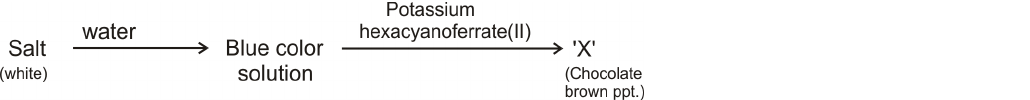
\includegraphics[width=0.95\linewidth]{Score-II - Test 32 (29 Mar 2024)-img/chem_q5_reaction.png}
\end{center}

if ppt.\ of 'x' is soluble in ammonia solution, and forms dark-blue solution of 'y' which contains two complex ion. Which of the following option is/are correct for 'y' solution?

\begin{qoptions}
\opt{A}{'y' is the solution of [Cu(CN)$_4$]$^{-2}$ and [Fe(CN)$_6$]$^{-3}$ ions.}
\opt{B}{One of the complex can show structural isomerism.}
\opt{C}{One of the complex ion in solution of 'y' produces blue ppt.\ with FeCl$_3$ solution.}
\opt{D}{One of the complex has tetrahedral geometry and other complex has octahedral geometry.}
\end{qoptions}

\textbf{6.} Toluene and benzene form an ideal solution over the whole range of composition. Two different solutions are made, solution I is one molal and solution II is two molal with respect to toluene. The vapour pressure of pure benzene is higher than that of pure toluene. The correct information(s) is/are:

\begin{qoptions}
\opt{A}{(V.P.)$_{\text{Solution-I}}$ = (V.P.)$_{\text{Solution-II}}$}
\opt{B}{(V.P.)$_{\text{Solution-I}}$ > (V.P.)$_{\text{Solution-II}}$}
\opt{C}{(V.P.)$_{\text{Solution-I}}$ < (V.P.)$_{\text{Solution-II}}$}
\opt{D}{Mole of benzene per kg solution is same in both solution.}
\end{qoptions}

\textbf{7.} The amino acid glycine (NH$_2$CH$_2$COOH) is basic because of its $-$NH$_2$ group and acidic because of its $-$COOH group. By a process equivalent to base dissociation, glycine can acquire an additional proton to form $^\oplus$NH$_3$CH$_2$COOH. The resulting cation may be considered to be a diprotic acid, since one proton from the $-$COOH group and one from the $-{}^\oplus$NH$_3$ group may be lost. The pK$_a$ values for these processes are 2.22 and 9.78, respectively. Select the correct statement(s) for a 0.01 M solution of neutral glycine (log 1.7 = 0.22, log 6 = 0.78),

\begin{qoptions}
\opt{A}{the pH is 6.0.}
\opt{B}{percentage of the glycine in the cationic form is 0.017\%.}
\opt{C}{the pOH is 6.0.}
\opt{D}{percentage of the glycine in the anionic form is 0.017\%.}
\end{qoptions}

\subsectionhdr{Section-II (i): Paragraph-based Numerical}

\textbf{Paragraph for Questions 1 and 2}

For the following reaction scheme, percentage yields are given along the arrow:

\end{multicols}
\begin{center}
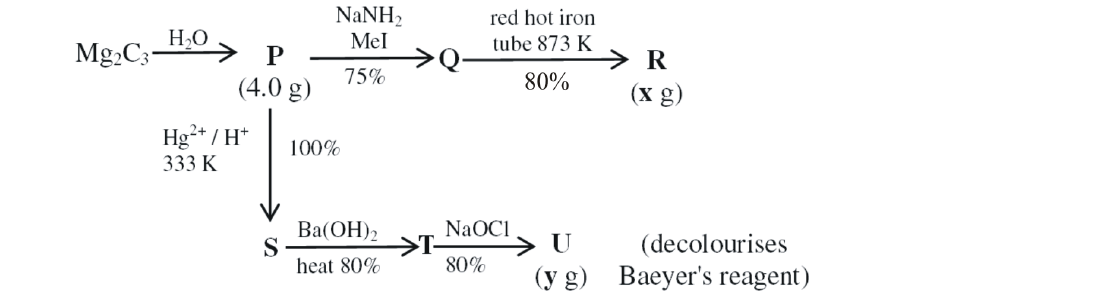
\includegraphics[width=0.75\linewidth]{Score-II - Test 32 (29 Mar 2024)-img/chem_p12_scheme.png}
\end{center}
\begin{multicols}{2}

\textbf{x} g and \textbf{y} g are mass of \textbf{R} and \textbf{U}, respectively. (Use: Molar mass (in g mol$^{-1}$) of H, C and O as 1, 12 and 16, respectively)

\textbf{1.} The value of \textbf{x} is\_\_\_\_\_.

\textbf{2.} The value of \textbf{y} is\_\_\_\_\_.

\textbf{Paragraph for Questions 3 and 4}

A black salt (A) is insoluble in dilute acid in cold but dissolve in boiling solution of concentrated hydrochloric acid, evolving a pungent smelling gas B. B turned a filter paper moistened with lead acetate, black. The above solution was cooled and separated into two parts. One part was treated with NaOH solution giving a white precipitate (C), insoluble in excess of reagent. C, when added to a concentrated H$_2$O$_2$ solution, a clear, yellowish-brown solution of D was formed. Other part of the original solution was treated with KI solution, giving a black precipitate (E), which dissolved in excess of reagent forming a clear orange solution.

\textbf{3.} Find the value of $|X-Y|$ where $X$ = sum of correct code, $Y$ = sum of incorrect code

\begin{itemize}[leftmargin=1.6em,itemsep=1pt,topsep=2pt]
\item[] Code-1 $\Rightarrow$ Hydroxide of cation in salt 'A' is soluble in excess of NH$_3$ solution
\item[] Code-2 $\Rightarrow$ When we add the hot H$_2$O in salt "E" then we get orange turbidity.
\item[] Code-3 $\Rightarrow$ In product "D" \& "E" central atom present in highest oxidation state.
\item[] Code-4 $\Rightarrow$ Salt "A" soluble in dil.\ HNO$_3$, conc.\ HCl \& also in aqua regia.
\item[] Code-5 $\Rightarrow$ When "B" react with BaCl$_2$ white ppt.\ will be formed.
\item[] Code-6 $\Rightarrow$ "B" can act as reducing agent while 'D' can act as oxidising agent.
\end{itemize}

\textbf{4.} Given the reaction scheme:

\begin{center}
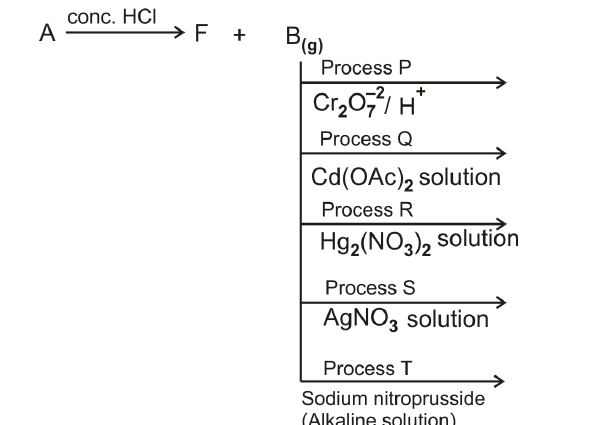
\includegraphics[width=0.95\linewidth]{Score-II - Test 32 (29 Mar 2024)-img/chem_p34_q4_scheme.png}
\end{center}

Number of process which produce colored ppt./turbidity/solution (except white/colorless).

\subsectionhdr{Section-II (ii): Non-negative Integer}

\textbf{5.} The number of sp$^2$ carbons in major product formed from the following reaction sequence is\_\_\_\_\_\_\_\_.

\end{multicols}
\begin{center}
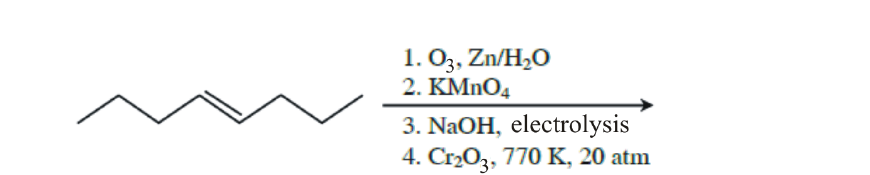
\includegraphics[width=0.65\linewidth]{Score-II - Test 32 (29 Mar 2024)-img/chem_n5_alkene.png}
\end{center}
\begin{multicols}{2}

\textbf{6.} The total number of chiral molecules formed from one molecule of \textbf{P} on complete ozonolysis (O$_3$, Zn/H$_2$O) is\_\_\_\_\_\_\_\_.

\end{multicols}
\begin{center}

\includegraphics[width=0.8\linewidth]{Score-II - Test 32 (29 Mar 2024)-img/chem_n6_structureP.png}
\end{center}
\begin{multicols}{2}

\textbf{7.} Consider the following reactions.
$$\text{NO}_2^\ominus\text{(aq.)} + \text{ClO}^-\text{(aq.)} \to \text{'X'(aq.)} + \text{Cl}^-\text{(aq.)}$$
$$\text{S(s)} + \text{ClO}^-\text{(aq.)} + \text{H}_2\text{O} \to \text{'Y'(aq.)} + \text{Cl}^-\text{(aq.)} + \text{H}^+\text{(aq.)}$$
Find the total atomicity of 'X' and 'Y' ions.

\textbf{8.} When 3 moles of XeO$_3$ react with NaOH in the presence of O$_3$ then it produce compounds 'A' \& 'B' only and 'B' when comes in contact with anhydrous CoCl$_2$ it turns pink. Then calculate the sum of moles of A \& B compounds.

\textbf{9.} For the electrochemical cell,
$$\text{Mg(s)}|\text{Mg}^{2+}(\text{aq, 1M})||\text{Cu}^{2+}(\text{aq, 1M})|\text{Cu(s)}$$
the standard emf of the cell is 2.70 V at 300 K. When the concentration of Mg$^{2+}$ is changed to x M, the cell potential changes to 2.67 V at 300 K. The value of x is\_\_\_\_. (given, $\dfrac{F}{R}=11500$ KV$^{-1}$, where F is the Faraday constant and R is the gas constant, $\ln(10)=2.30$)

\textbf{10.} If Pd v/s P (where P denotes pressure in atm and d denotes density in gm/L) is plotted for H$_2$ gas (ideal gas) at a particular temperature. If $\left[\dfrac{d}{dP}(Pd)\right]_{P=8.21\,\text{atm}}=10$, then the temperature (in K) will be

\sectionhdr{PART-3: MATHEMATICS}
\subsectionhdr{Section-I (i): Single Correct}

\textbf{1.} Consider the polynomial $P(x) = x^3 + ax^2 + bx + c$ where $a, b, c \in \{1, 2, \ldots, 10\}$ then the probability that $P(x)$ is divisible by $x^2 + x + 1$ is

\begin{qoptions}
\opt{A}{$\dfrac1{100}$}
\opt{B}{$\dfrac9{1000}$}
\opt{C}{$\dfrac1{1000}$}
\opt{D}{$\dfrac9{100}$}
\end{qoptions}

\textbf{2.} If p and q are prime numbers and the equation $x^2 - px + q = 0$ has distinct integral roots then which of the following statements are true

I : The difference of the roots is odd\\
II : Atleast one root is prime\\
III : $p^2 - q$ is prime\\
IV : $p + q$ is prime

\begin{qoptions}
\opt{A}{I only}
\opt{B}{II only}
\opt{C}{II and III only}
\opt{D}{All are true}
\end{qoptions}

\textbf{3.} The value of the definite integral $\displaystyle\int_{\pi/8}^{3\pi/8}\dfrac{11+4\cos2x+\cos4x}{1-\cos4x}\,dx$ equals

\begin{qoptions}
\opt{A}{$-6-\dfrac\pi4$}
\opt{B}{$6\sqrt2-\dfrac\pi4$}
\opt{C}{$12-\dfrac\pi2$}
\opt{D}{$6-\dfrac\pi4$}
\end{qoptions}

\textbf{4.} The normals at P and Q on a parabola $y^2 = 4ax$ intersect at a point R on the curve. If M is the mid point of PQ and N is the mid point of MR, then locus of N is

\begin{qoptions}
\opt{A}{$y^2=a(x-a)$}
\opt{B}{$y^2=3a(x+a)$}
\opt{C}{$3y^2=a(x+a)$}
\opt{D}{$3y^2=a(x-a)$}
\end{qoptions}

\subsectionhdr{Section-I (ii): One or more correct}

\textbf{5.} Let $f(x)$ be a decreasing function and positive for all x and an ellipse be $\dfrac{x^2}{f(k^2+2k+5)}+\dfrac{y^2}{f(k+11)}=1$.

\begin{qoptions}
\opt{A}{If x axis is major axis of ellipse, then $k\in(-3,2)$.}
\opt{B}{If x axis is major axis of ellipse, then $k\in(-\infty,-3)\cup(2,\infty)$.}
\opt{C}{If y axis is major axis of ellipse, then $k\in(-3,2)$.}
\opt{D}{If y axis is major axis of ellipse, then $k\in(-\infty,-3)\cup(2,\infty)$.}
\end{qoptions}

\textbf{6.} Let A be a square matrix of order 3 such that $\text{Tr.}(A^{-1})=3$ and $\det(A^{-1})=\dfrac15$. If $(A^{-1}B^{-1}A)^{-1}=2(\text{adj }A)$, then

[Note: Tr.(P) and adj P denote trace of square matrix P and adjoint matrix of square matrix P respectively.]

\begin{qoptions}
\opt{A}{$\det(B)=5000$}
\opt{B}{$\det(B)=200$}
\opt{C}{$\text{Tr.}(B)=30$}
\opt{D}{$\text{Tr.}(B)=15$}
\end{qoptions}

\textbf{7.} If $^{100}C_{50}$ can be prime factorised as $2^\alpha\cdot3^\beta\cdot5^\gamma\cdot7^\delta\ldots\ldots$ where $\alpha,\beta,\gamma,\delta\ldots\ldots$ are non-negative integers, then correct relation is/are

\begin{qoptions}
\opt{A}{$\alpha<\beta$}
\opt{B}{$\gamma<\delta$}
\opt{C}{$\alpha+\delta=\beta+\gamma-1$}
\opt{D}{$\gamma+\delta=0$}
\end{qoptions}

\subsectionhdr{Section-II (i): Paragraph-based Numerical}

\textbf{Paragraph for Questions 1 and 2}

ABCD is a square of side length 2 units and the centre of square is at origin. $C_2$ is a circle passing through vertices A, B, C, D and $C_1$ is the circle touching all the sides of square ABCD. Line $L_1$ is tangent at A and line $L_2$ is tangent at D on circle $C_2$ respectively which intersects at K, where A, B, C, D lie in $2^{\text{nd}}$, $1^{\text{st}}$, $4^{\text{th}}$, $3^{\text{rd}}$ quadrant respectively. Point Q is variable point on $C_2$ let perpendicular drawn from Q to cut the line $L_1$ and $L_2$ at E and F respectively. Given that AB, BC, CD and AD are parallel to the coordinate axes.

\textbf{1.} The maximum area of rectangle QEKF is\_\_\_\_\_\_\_\_.

\textbf{2.} Area of $\triangle BQC$, (where Q is such that the area of the rectangle QEKF is maximum) is\_\_\_\_\_\_\_\_.

\textbf{Paragraph for Questions 3 and 4}

Consider, an ellipse and hyperbola as given $H:\dfrac{x^2}{a^2}-\dfrac{y^2}3=1$ and $E:\dfrac{x^2}{4a^2}+\dfrac{y^2}9=1$. If both the curves are orthogonal to each other and $e_H$ and $e_E$ are eccentricities of hyperbola and ellipse respectively, then

\textbf{3.} The value of $|a|$ is\_\_\_\_\_\_\_\_.

\textbf{4.} Area of the quadrilateral formed by two pair of tangents drawn to the hyperbola from $(1,0)$ and to the ellipse from $(5,0)$ is\_\_\_\_\_\_\_\_.

\subsectionhdr{Section-II (ii): Non-negative Integer}

\textbf{5.} The sequence $\{a_n\}_{n=1}^{+\infty}$ is defined by $a_1=0$ and $a_{n+1}=a_n+4n+3,\ n\geq1$. Find the value of
$$\lim_{n\to\infty}\dfrac{\sqrt{a_n}+\sqrt{a_{4n}}+\sqrt{a_{4^2n}}+\sqrt{a_{4^3n}}+\ldots+\sqrt{a_{4^{10}n}}}{\sqrt{a_n}+\sqrt{a_{2n}}+\sqrt{a_{2^2n}}+\sqrt{a_{2^3n}}+\ldots+\sqrt{a_{2^{10}n}}}$$
equals

\textbf{6.} Number of continuously differentiable function $f:\mathbb R\to\mathbb R$ satisfying $f(x)>0$ and $f'(x)=f(f(x))\ \forall x\in\mathbb R$ is/are

\textbf{7.} Raman has two dice. One die has three faces marked with 1; two faces marked with 2 and one face marked with 3, another die has one face marked with 1, two faces marked with 2 and three marked with 3, then the maximum probability of getting a sum of 4 on two dice is $\dfrac mn$, where m and n are coprime then value of $(m+n)$ is\_\_\_\_\_\_\_\_.

\textbf{8.} Let $S_1:x^2+y^2+4x-6y-12=0$ and $S_2:x^2+y^2-3x-2y+1=0$ be two circles with centres $C_1$ and $C_2$ respectively. If A and B are two points which lie on their common chord as well as common tangents and $C_1A^2-C_2A^2=\dfrac ab$, where $a,b\in\mathbb N$, then find least value of $(a-22b)$.

\textbf{9.} If $\vec a=x\hat i+y\hat j+2\hat k$, $\vec b=\hat i-\hat j+\hat k$, $\vec c=\hat i+2\hat j$ and $\vec a\wedge\vec b=\dfrac\pi2$, $\vec a\cdot\vec c=4$.

Find the value of scalar triple product
$$\resizebox{\linewidth}{!}{$\left[\left(\dfrac{\vec a+2\vec b-\vec c}2\right)\left(\dfrac{\vec a-\vec b}2\right)\left(\dfrac{\vec a-\vec b-\vec c}2\right)\right]$}$$

\textbf{10.} If $n_1,n_2,n_3\ldots\ldots n_{100}$ are positive real numbers such that $n_1+n_2+n_3+\ldots\ldots+n_{100}=20$ and $k=n_1(n_2+n_3+n_4)(n_5+n_6+\ldots\ldots n_9)(n_{10}+\ldots\ldots n_{16})\ldots\ldots(\ldots\ldots+n_{100})$, then find the sum of digits of maximum value of k.

\end{multicols}
\end{document}
